\begin{enumerate}
	\item On choisit $1$ comme nombre de départ :\qquad
	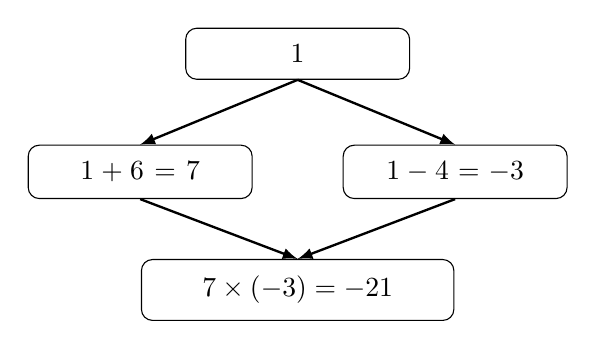
\begin{tikzpicture}[every node/.style={align=center,inner ysep=6pt,inner xsep=12pt,minimum width=2cm, rounded corners}, baseline={(a.base)}]
	\node(a)at(0,0)[text width=2cm,draw]{1};
	\node(b)at(-2,-1.5)[text width=2cm,draw]{{$1+6=7$}};
	\node(c)at(2,-1.5)[text width=2cm,draw]{{$1-4=-3$}};
	\node(d)at(0,-3)[draw]{\quad$7\times(-3)=-21$\quad};
	\draw[->,>=latex,line width=0.3mm](a.south)--(b.north);
	\draw[->,>=latex,line width=0.3mm](a.south)--(c.north);
	\draw[->,>=latex,line width=0.3mm](b.south)--(d.north);
	\draw[->,>=latex,line width=0.3mm](c.south)--(d.north);	\end{tikzpicture}

	Si on choisit $1$, on obtient effectivement $-21$ avec le programme A.

	\item {$10\xrightarrow{\text{élever au carré}}10^2=100$\quad puis \quad $100 \xrightarrow{\text{soustraire }9}100-9=91$}

	Avec le programme B, on obtient $91$ lorsque le nombre de départ est $10$.

	\item Si on choisit $x$ comme nombre de départ, le programme B calcule {$x^2-9$}.

	On cherche donc pour quelle(s) valeur(s) de $x$ on obtient $16$,

	autrement dit \quad {$x^2-9=16\iff x^2-25=0$}.

	On remarque que {$25=5^2$}, donc on peut factoriser une identité remarquable et l'équation à résoudre devient {$(x-5)(x+5)=0$.}

	Un produit est nul si et seulement si un des facteurs est nul; donc il y a deux solutions qui sont $-5$ et $5$.

	Si on choisit un de ces deux nombres, on obtiendra $16$ avec le programme B.

	\item \begin{minipage}[t]{0.45\linewidth} Ligne 3, on ajoute 6, ligne 4, on soustrait 4 et enfin ligne 5 on fait le produit des 2 résultats intermédiaires.
	\end{minipage}\hfill~
	\begin{scratch}[num blocks,num start=3, baseline=3]
	\blockvariable{mettre \selectmenu{Valeur 1} à  {\ovaloperator{\ovalsensing{réponse} + \ovalnum{6}}}}
	\blockvariable{mettre \selectmenu{~Valeur 2} à  {\ovaloperator{\ovalsensing{réponse} - \ovalnum{4}}}}
	\blockvariable{mettre \selectmenu{Résultat} à  \ovaloperator{\ovalvariable{Valeur 1} ~* \ovalvariable{Valeur 2}}}
	\end{scratch}\hfill~
	\item On choisit $x$ comme nombre de départ dans le programme A :

	\begin{center}
		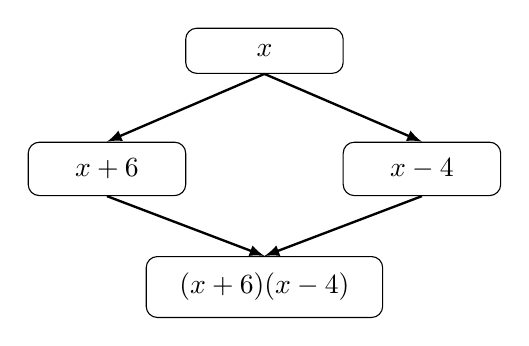
\begin{tikzpicture}[every node/.style={align=center,inner ysep=6pt,inner xsep=12pt,minimum width=2cm, rounded corners}, baseline={(a.base)}]
	\node(a)at(0,0)[draw]{$x$};
	\node(b)at(-2,-1.5)[draw]{{$x+6$}};
	\node(c)at(2,-1.5)[draw]{{$x-4$}};
	\node(d)at(0,-3)[draw]{$(x+6)(x-4)$};
	\draw[->,>=latex,line width=0.3mm](a.south)--(b.north);
	\draw[->,>=latex,line width=0.3mm](a.south)--(c.north);
	\draw[->,>=latex,line width=0.3mm](b.south)--(d.north);
	\draw[->,>=latex,line width=0.3mm](c.south)--(d.north);	\end{tikzpicture}
	\end{center}

	On développe : \quad {$(x+6)(x-4)=x^2-4x+6x-24=x^2+2x-24$}.

	Avec le programme A, on calcule {$x^2+2x-24$}.

	\item On sait que le programme A calcule \quad {$x^2+2x-24$} \quad et le programme B \quad {$x^2-9$}.

	Les deux programmes donnent le même résultat si et seulement si \quad {$x^2+2x-24=x^2-9$}.

	Cette équation peut se simplifier en soustrayant $x^2$ à chaque membre, et elle devient :

	$\begin{aligned}
			2x-24=-9&\iff2x=15\\&\iff x=\dfrac{15}{2}
		\end{aligned}$

	Les deux programmes donnent le même résultat si on choisit comme nombre de départ {$\dfrac{15}{2}=\np{7.5}$} et ce résultat est \np{47.25}.
\end{enumerate}
